\section*{Introduction}
\frame{
    \center \LARGE{Introduction}
}

\begin{frame}
    \frametitle{Linux ?}
        \begin{itemize}
            \item<1 -> Linux est un \textbf{noyau} et non un \textbf{système d'exploitation}
            \item<2 -> Système d'exploitation (GNU/Linux) = Espace Utilisateur (GNU) + Noyau (Linux)
        \end{itemize}
\end{frame}

\begin{frame}
        \begin{center}
            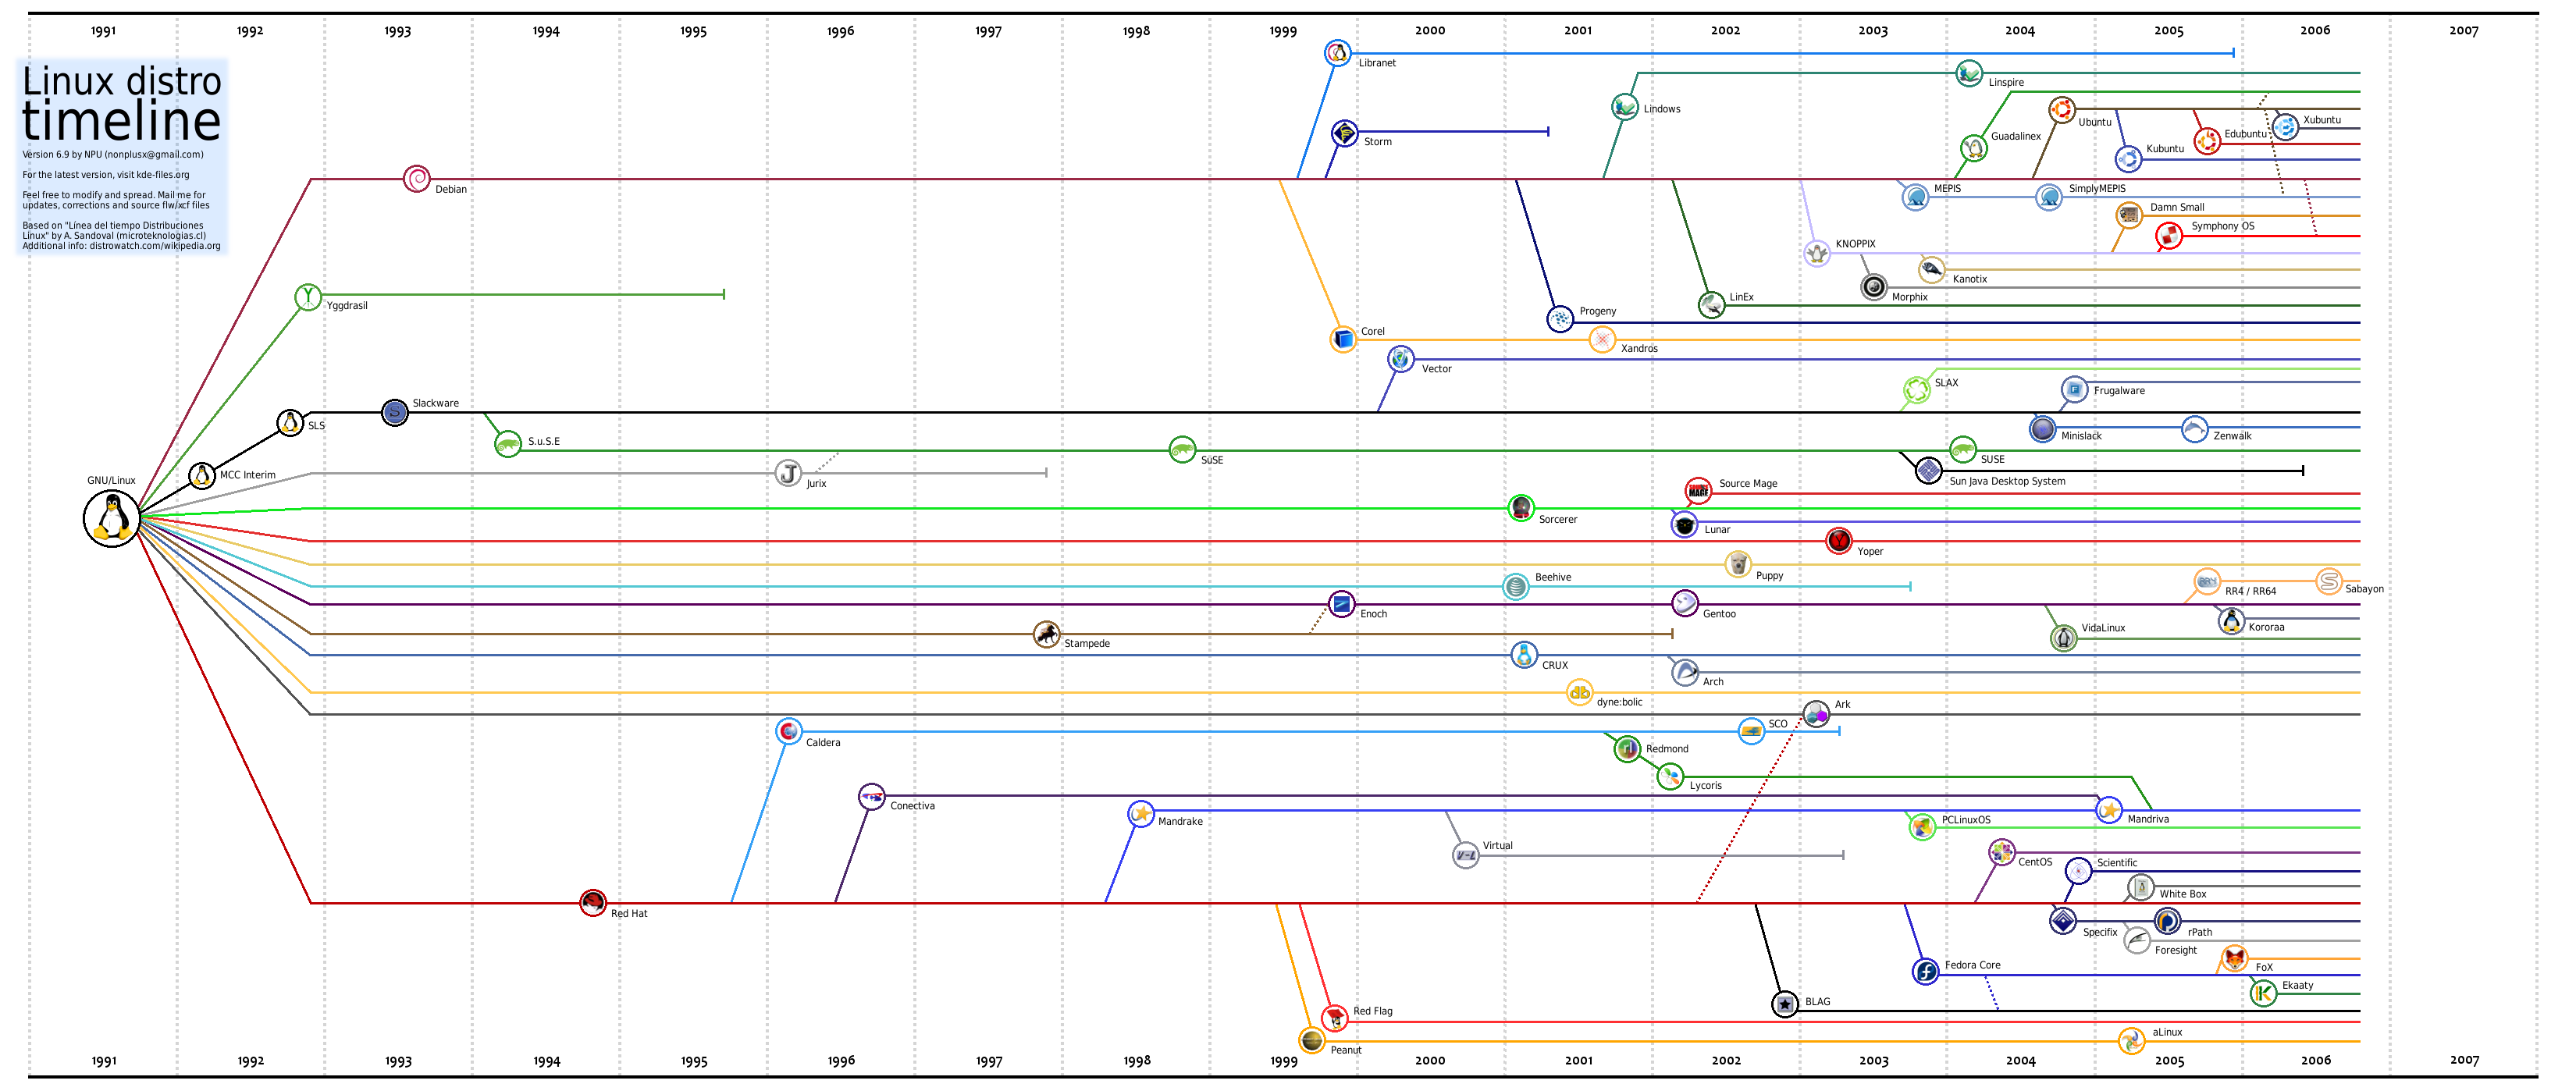
\includegraphics[width=\linewidth, height=\textheight, keepaspectratio]{linux_timeline.png}
        \end{center}
\end{frame}
